%%%%%%%%%%%%%%%%%%%%%%%%%%%%%%%%%%%%%%%%%%%%%%%%%%%%%%%%%%%%%%%%%%%%%%%%%%%%%%%%
%2345678901234567890123456789012345678901234567890123456789012345678901234567890
%        1         2         3         4         5         6         7         8


\documentclass[a4paper, 10pt, conference] {article}        
                                                           

%\IEEEoverridecommandlockouts                              % This command is only
                                                          % needed if you want to
                                                          % use the \thanks command
%\overrideIEEEmargins
% See the \addtolength command later in the file to balance the column lengths
% on the last page of the document



% The following packages can be found on http:\\www.ctan.org
\usepackage{graphicx} % for pdf, bitmapped graphics files
\usepackage{caption}
\usepackage{float}
\usepackage{subcaption}
\usepackage{epsfig} % for postscript graphics files
\usepackage{mathptmx} % assumes new font selection scheme installed
\usepackage{times} % assumes new font selection scheme installed
\usepackage{amsmath} % assumes amsmath package installed
\usepackage{amssymb}  % assumes amsmath package installed
\usepackage[margin=1.5cm]{geometry}
\usepackage{mathtools}
%\usepackage{enumerate}
\usepackage{enumitem}
\usepackage{lipsum}
\begin{document}
\date{}
\title{\LARGE \bf
B31SE2 – Matlab Lab 1
Fourier Theory. Image Analysis in Frequency Domain
}

\author{ \parbox{5 in}{\centering Daniel Barmaimon \\
%         \thanks{*Use the $\backslash$thanks command to put information here}\\
         \ Advanced Image Analysis - Vibot Master Degree\\
         \ Heriot Watt University\\         
}}

\maketitle
%\thispagestyle{empty}
%\pagestyle{empty}


\section{Introduction}
In this lab is presented the problem of restoring an image that has been corrupted by certain blur and additionally has some noise. One of the most common ways of thinking about this problem is by finding the mathematical model and minimizing the energy. The simple model could be found as the equation below. 
\begin{equation}
g(x,y) = H[f(x,y)]+ n(x,y) 	
\end{equation} 
Where \textit{$f(x,y)$} is the original image, \textit{$n(x,y)$} is the model of the noise, and \textit{$H$} is a linear operator that represents the transformation for blurring the image.
The two kernels that are going to be used during this lab are Gaussian and motion, and could be seen in Fig.\ref{kern}
\begin{figure}[H]
 	\centering
 	\begin{subfigure}{0.49\textwidth} 
 		\centering						
 		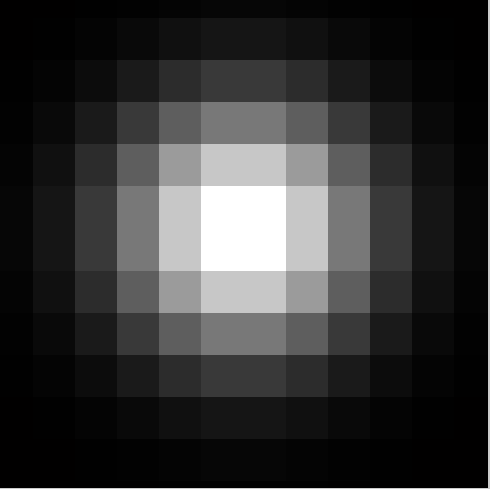
\includegraphics[scale=0.3]{gaussian/no_noise/kernel_sigma2.PNG}
		\caption{Gaussian kernel}
	\end{subfigure}
	\begin{subfigure}{0.49\textwidth}
		\centering
		
\includegraphics[scale=0.3]{motion/kernel_alpha30.PNG}
		\caption{Motion kernel}
	\end{subfigure}
	\caption{Kind og kernels for blurring the image}
	\label{kern}
\end{figure}


As \textit{$H$} is a convolution the blurred image could be expressed as follows. 
\begin{equation}
g(x,y) = \iint h(x-u, y-v) \cdot f(u,v) \cdot dudv + n(x,y)
\end{equation}
For reasons of computation it recommendable to transform this equation to the frequency domain having as result the following expression.
\begin{equation}
G(u,v) = H(u,v) \cdot F(u,v) + N(u,v)
\end{equation}

\section{Fundamentals}
The idea to solve the deblurring problem could be related with a minimization one. The following approach is called variational regularization for image deblurring.
\begin{enumerate} %[leftmargin=2.5cm]
	\item Find the energy
	In this lab, we will find the minimum for to different energies.
	\begin{enumerate}
		\item $\left|\left|  h\otimes f - g \right|\right|^{2} + \mu \cdot \left| \left|f \right|\right|^{2} $ 
		\item $\left|\left|  h\otimes f - g \right|\right|^{2} + \mu \cdot \left| \left|\bigtriangledown f \right|\right|^{2} $
 	\end{enumerate}
 	where $\mu $ is the approximation of the quotient of the power spectrum of noise divided by the power spectrum of the non-degraded image (noise to signal ratio).\\
 	It's important to recall that the main difference in the methods is that the first energy tries to restore the image itself while the second energy tries to restore the image edges.
	 
	\item Calculate the gradient of the energy $\bigtriangledown E$ 
	
	\item Minimize the energy
 	
\end{enumerate}

\section{Analysis and results}
\subsection{ Deblurring images without noise}
The first experiment to perform is related with recovering a blurred imaged once we know the kernel that has degraded it. Let's start analyzing the first energy and how the recovered image looks after applying different values for the parameter $ \lambda = 1 / \mu$. The original image and the blurred image could be seen at Fig.\ref{noNoiseOriginal} and the results varying the $\lambda$ parameter are shown in Fig.\ref{noNoiseRecovered}

\begin{figure}[H]
	\centering
	\begin{subfigure}{0.49\textwidth} 
		\centering						
		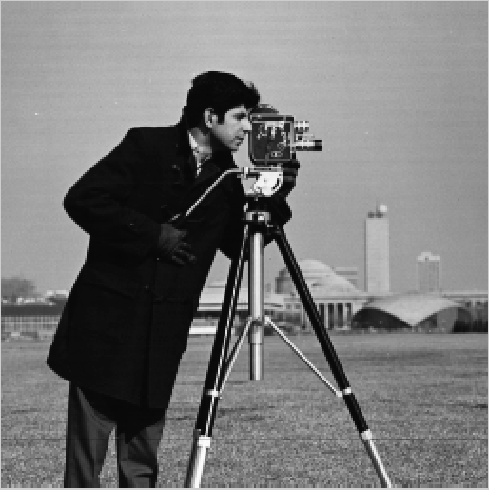
\includegraphics[scale=0.48]{gaussian/no_noise/original.PNG}
		\caption{Original image}
	\end{subfigure}
	\begin{subfigure}{0.49\textwidth}
		\centering
		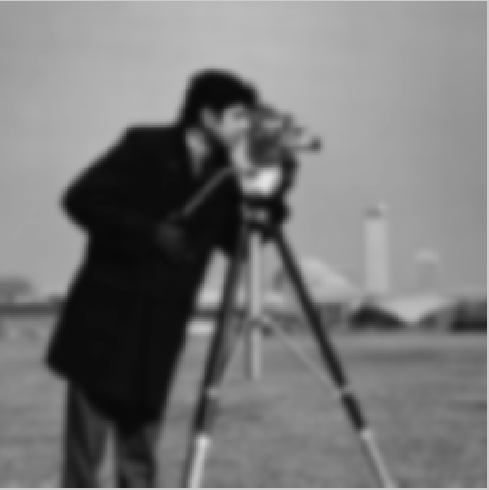
\includegraphics[scale=0.48]{gaussian/no_noise/blurred_sigma2.PNG}
		\caption{Blurred image with Gaussian kernel ($\sigma = 2$)}
	\end{subfigure}
	\caption{Restored images with different $\lambda$}
	\label{noNoiseOriginal}
\end{figure}

\begin{figure}[H]
	\centering
	\begin{subfigure}{0.49\textwidth} 
		\centering						
		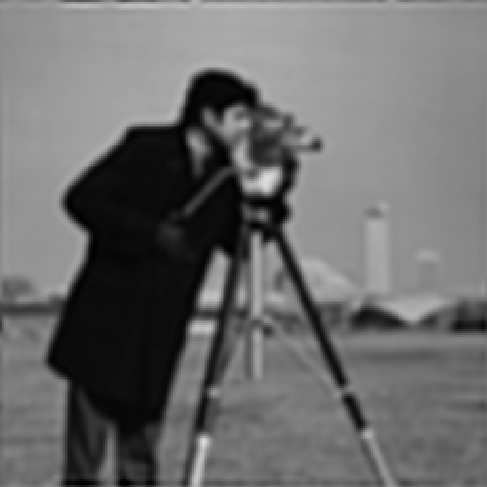
\includegraphics[scale=0.48]{gaussian/no_noise/lam10.PNG}
		\caption{$\lambda = 10$}
	\end{subfigure}
	\begin{subfigure}{0.49\textwidth} 
		\centering						
		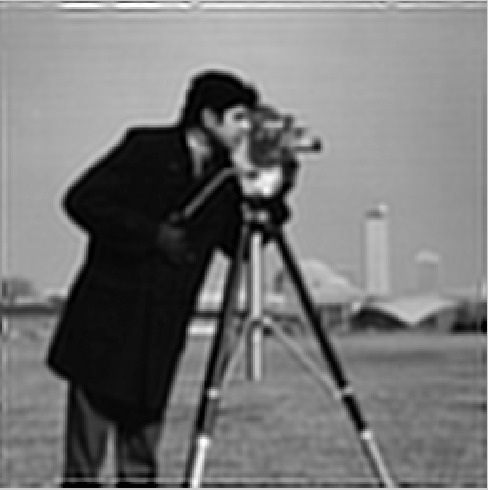
\includegraphics[scale=0.48]{gaussian/no_noise/lam100.PNG}
		\caption{$\lambda = 100$}
	\end{subfigure}\\
	\begin{subfigure}{0.49\textwidth} 
		\centering						
		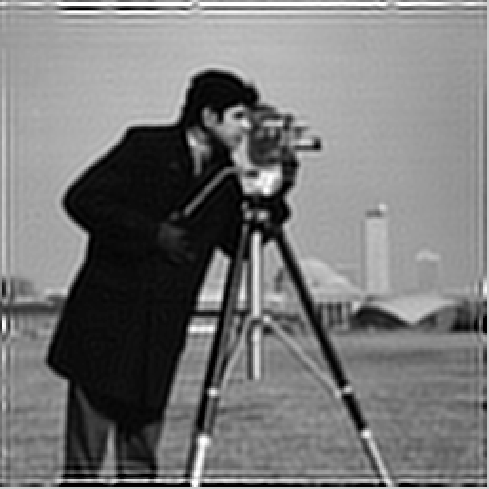
\includegraphics[scale=0.48]{gaussian/no_noise/lam1000.PNG}
		\caption{$\lambda = 1000$}
	\end{subfigure}
	\begin{subfigure}{0.49\textwidth} 
		\centering						
		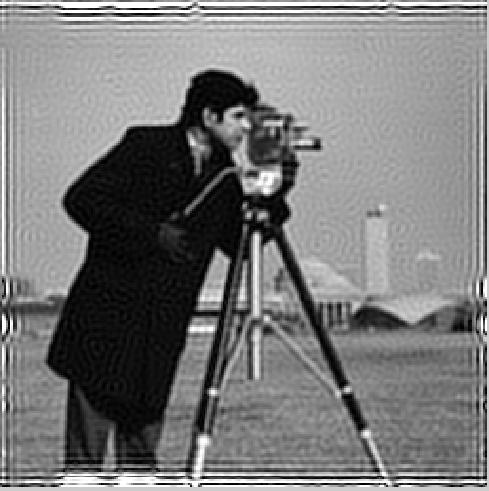
\includegraphics[scale=0.48]{gaussian/no_noise/lam10000.PNG}
		\caption{$\lambda = 10000$}
	\end{subfigure}
	\caption{Restored images with different $\lambda$}
	\label{noNoiseRecovered2}
\end{figure}
It could be appreciated that the higher is the value of lambda the clearer are the edges on the recovered image. But, in the images where $\lambda = 1000$ and $\lambda = 10000$ some artifacts appear. Also the negative effect over the boarders of the images are increased with higher values of $\lambda$. It could be partially avoided choosing 'circular' and 'conv' as when defining the kernel ('circular' for periodic implementation, 'conv' for multidimensional filter as this case).

\begin{figure}[H]
	\centering
	\begin{subfigure}{0.49\textwidth} 
		\centering						
		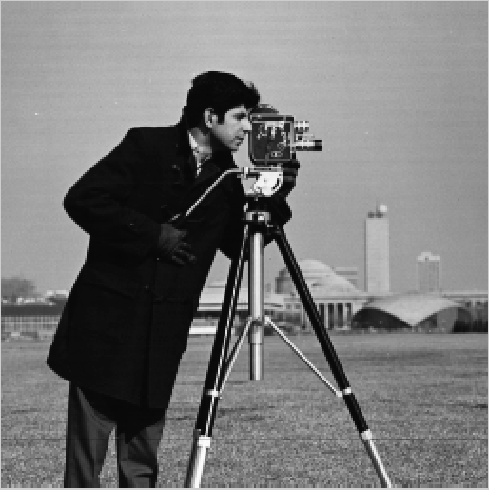
\includegraphics[scale=0.48]{gaussian/no_noise/original.PNG}
		\caption{Original image}
	\end{subfigure}
	\begin{subfigure}{0.49\textwidth}
		\centering
		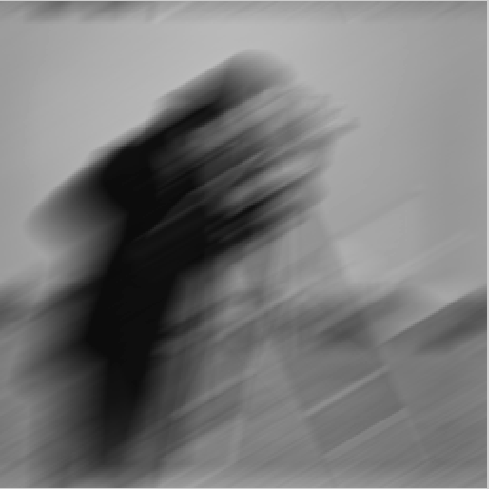
\includegraphics[scale=0.48]{motion/no_noise/blured_len50_alpha30.PNG}
		\caption{Blurred image with motion kernel ($length = 50$, $\alpha = 30º$)}
	\end{subfigure}
	\caption{Original and blurred images (without noise)}
	\label{noNoiseOriginal2}
\end{figure}

\begin{figure}[H]
	\centering
	\begin{subfigure}{0.49\textwidth} 
		\centering						
		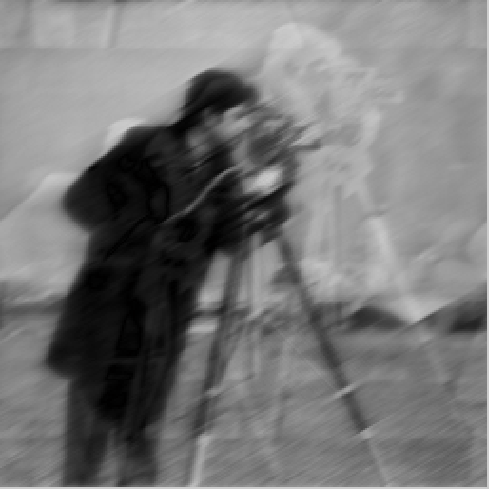
\includegraphics[scale=0.48]{motion/no_noise/lam100.PNG}
		\caption{$\lambda = 100$}
	\end{subfigure}
	\begin{subfigure}{0.49\textwidth} 
		\centering						
		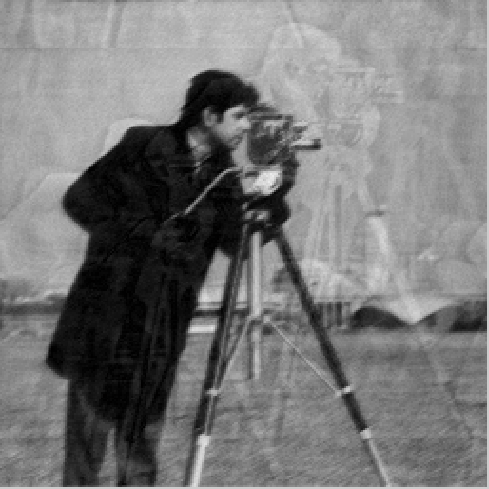
\includegraphics[scale=0.48]{motion/no_noise/lam1000.PNG}
		\caption{$\lambda = 1000$}
	\end{subfigure}\\
	\begin{subfigure}{0.49\textwidth} 
		\centering						
		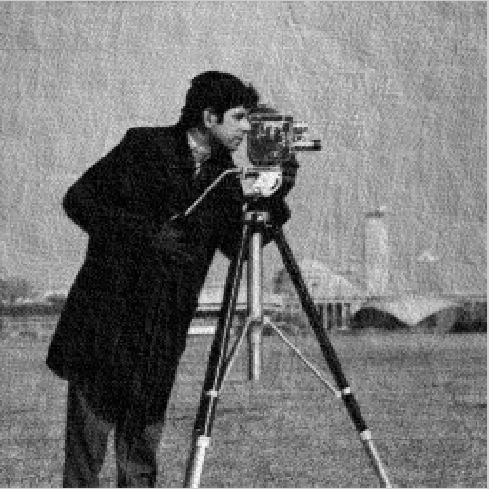
\includegraphics[scale=0.48]{motion/no_noise/lam10000.PNG}
		\caption{$\lambda = 10000$}
	\end{subfigure}
	\begin{subfigure}{0.49\textwidth} 
		\centering						
		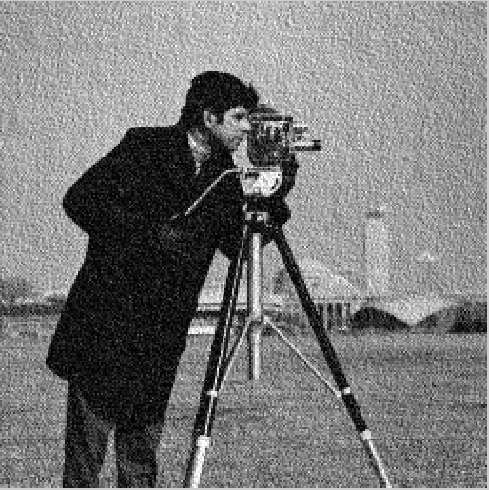
\includegraphics[scale=0.48]{motion/no_noise/lam100000.PNG}
		\caption{$\lambda = 100000$}
	\end{subfigure}
	\caption{Original and blurred images (without noise)}
	\label{noNoiseRecovered}
\end{figure}
In the case of the motion blur, is important to take care of the size of the kernel that is not going to coincide with the size of the image. That is a problem if it is wanted to use the multiplication of element by element in the Fourier domain to avoid the convolution computation in the space domain. To solve this problem the function \textit{psf2otf} is used. It converts the PSF array into an OTF array, and for our application the same size of the input image is set as parameter.\\
It could be observed in Fig.\ref{noNoiseRecovered2} that there are some 'phantoms' with the silhouette of the photographer in the direction of the kernel. The higher is the parameter $\lambda$, the lower is this effect(cases (a) and (b)). But for very high values of this parameter new artifacts appear (cases (c) and (d)).  

\subsection{Deblurring images with noise}
In this section the intention is to check how different kind of noise (gaussian, salt and pepper, speckle) affects to the performance of the deblurring techniques.
\begin{figure}[H]
	\centering
	\begin{subfigure}{0.49\textwidth} 
		\centering						
		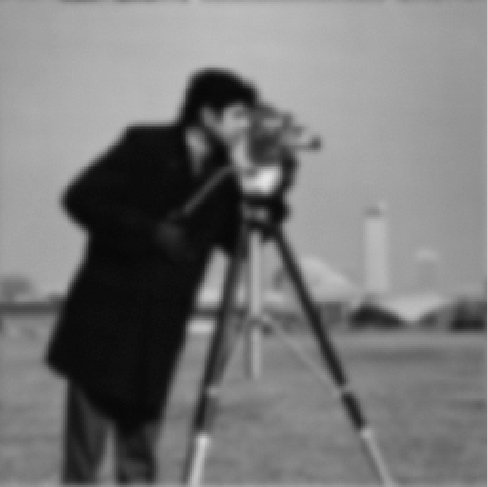
\includegraphics[scale=0.48]{gaussian/noisy/gaussian_00001.PNG}
		\caption{Gaussian noise $\sigma = 10^{-5}$}
	\end{subfigure}
	\begin{subfigure}{0.49\textwidth} 
		\centering						
		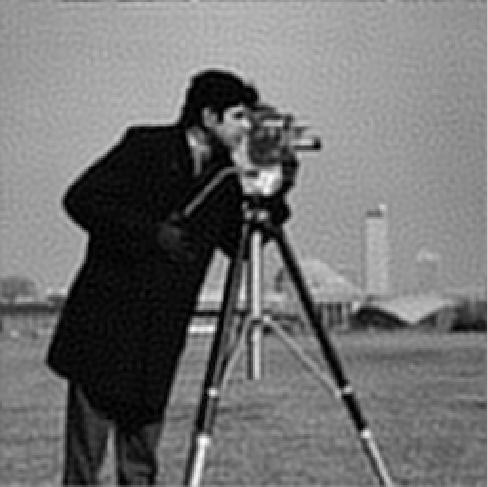
\includegraphics[scale=0.48]{gaussian/noisy/recovered_gaussian_00001_lam1000.PNG}
		\caption{Recovered with $\lambda = 1000$}
	\end{subfigure}\\
	\begin{subfigure}{0.49\textwidth} 
		\centering						
		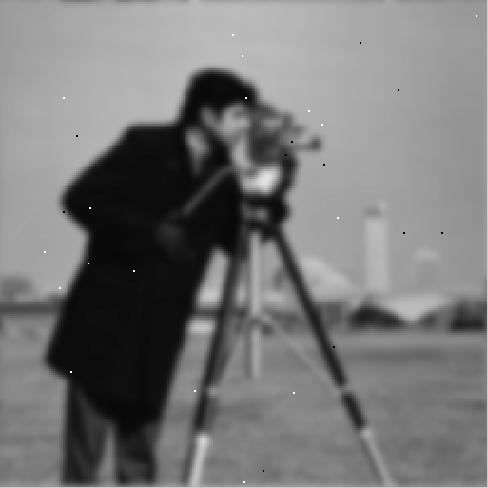
\includegraphics[scale=0.48]{gaussian/noisy/saltpepper0005.PNG}
		\caption{Salt \& pepper $d =5\cdot 10^{-4}$}
	\end{subfigure}
	\begin{subfigure}{0.49\textwidth} 
		\centering						
		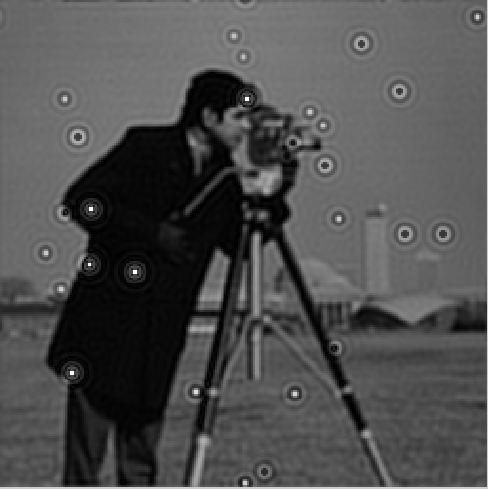
\includegraphics[scale=0.48]{gaussian/noisy/recovered_saltpepper0005.PNG}
		\caption{Recovered with $\lambda = 1000$}
	\end{subfigure}
	\begin{subfigure}{0.49\textwidth} 
		\centering						
		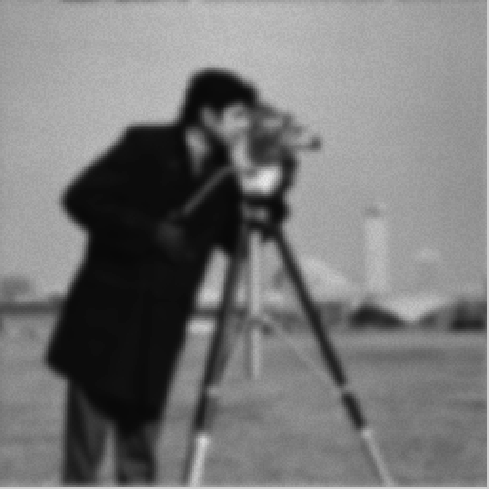
\includegraphics[scale=0.48]{gaussian/noisy/speckle0004.PNG}
		\caption{Speckle noise $d =4\cdot 10^{-4}$}
	\end{subfigure}
	\begin{subfigure}{0.49\textwidth} 
		\centering						
		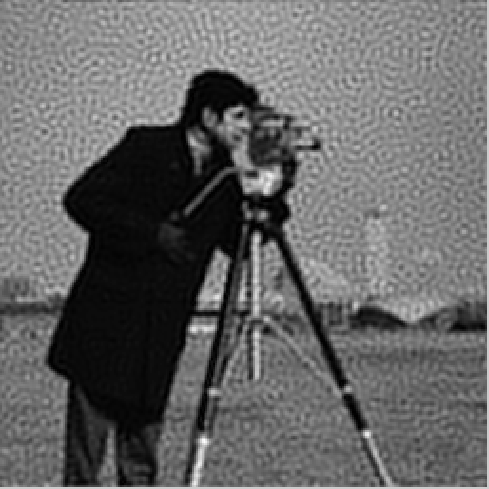
\includegraphics[scale=0.48]{gaussian/noisy/recovered_speckle0004.PNG}
		\caption{Recovered with $\lambda = 1000$}
	\end{subfigure}
	\caption{Noisy and recovered images for Gaussian kernel}
	\label{noisy1}
\end{figure}
The case of Gaussian noise is the only one that doesn't project any artifact when recovering the original image. It is specially bad for salt \& pepper noise where the dots are converted into little Gaussian distributions and degrade the image much more than the other two cases.

\begin{figure}[H]
	\centering
	\begin{subfigure}{0.49\textwidth} 
		\centering						
		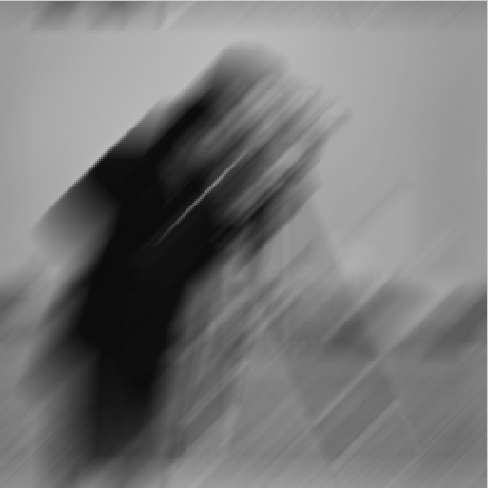
\includegraphics[scale=0.48]{motion/noisy/gaussian_000001.PNG}
		\caption{Gaussian noise $\sigma = 10^{-6}$}
	\end{subfigure}
	\begin{subfigure}{0.49\textwidth} 
		\centering						
		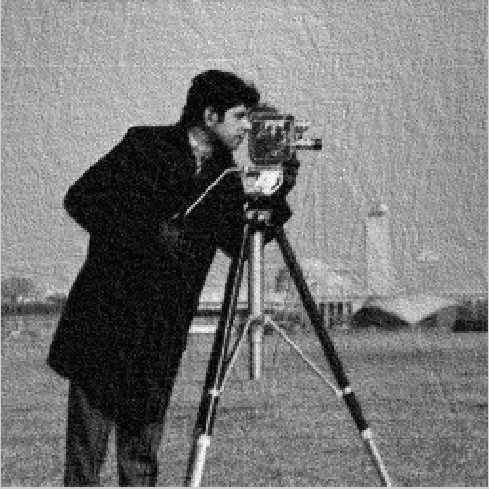
\includegraphics[scale=0.48]{motion/noisy/recovered_gaussian_000001_lam7500.PNG}
		\caption{Recovered with $\lambda = 7500$}
	\end{subfigure}\\
	\begin{subfigure}{0.49\textwidth} 
		\centering						
		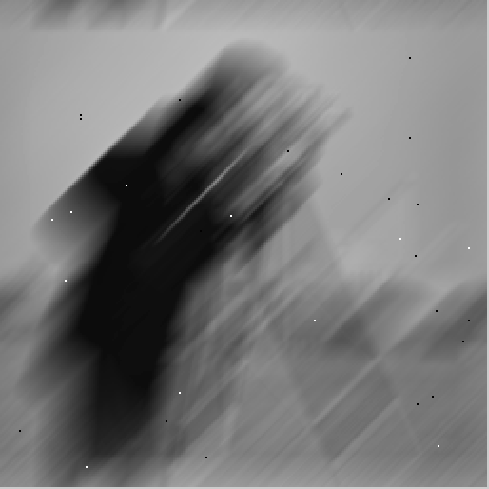
\includegraphics[scale=0.48]{motion/noisy/saltpepper00005.PNG}
		\caption{Salt \& pepper $d =5\cdot 10^{-4}$}
	\end{subfigure}
	\begin{subfigure}{0.49\textwidth} 
		\centering						
		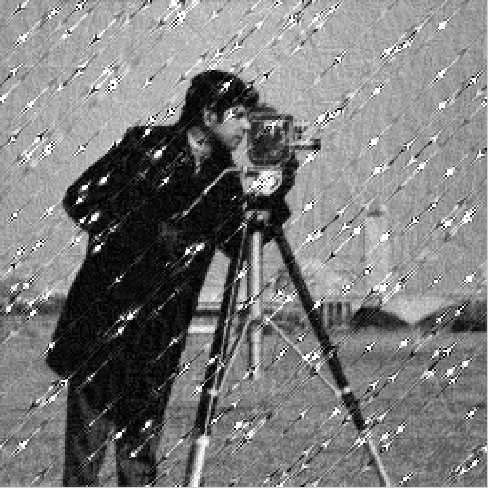
\includegraphics[scale=0.48]{motion/noisy/recovered_saltpepper00005.PNG}
		\caption{Recovered with $\lambda = 7500$}
	\end{subfigure}
	\begin{subfigure}{0.49\textwidth} 
		\centering						
		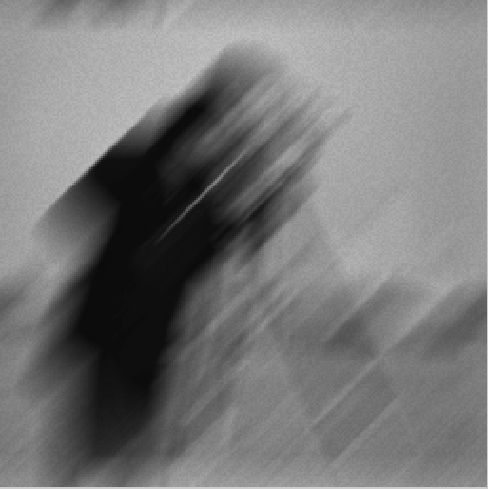
\includegraphics[scale=0.48]{motion/noisy/speckle_d00004.PNG}
		\caption{Speckle noise $d =4\cdot 10^{-4}$}
	\end{subfigure}
	\begin{subfigure}{0.49\textwidth} 
		\centering						
		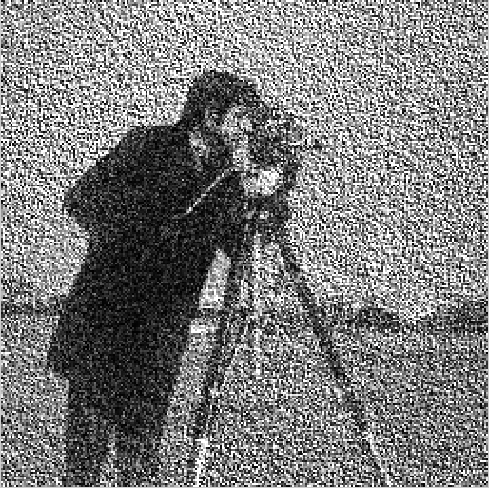
\includegraphics[scale=0.48]{motion/noisy/recovered_speckle_d00004.PNG}
		\caption{Recovered with $\lambda = 7500$}
	\end{subfigure}
	\caption{Noisy and recovered images for motion kernel}
	\label{noisy2}
\end{figure}
In the case of motion blur image, and setting properly (if not artifacts like in S \& P appear) the parameter $\lambda$ is possible to recover a nice image of Gaussian and salt and pepper noise if it is low density. In the case of speckle noise is quite difficult to recover the original image.

\subsection{Comparison of the two energies}
In this last section the two different energies would be compared. Apparently there is no big differences for the two energies as could be observed in the images of Fig.\ref{comparison1} 
It was used lambda = 500, in both of the cases.
\begin{figure}[H]
	\centering
	\begin{subfigure}{0.49\textwidth} 
		\centering						
		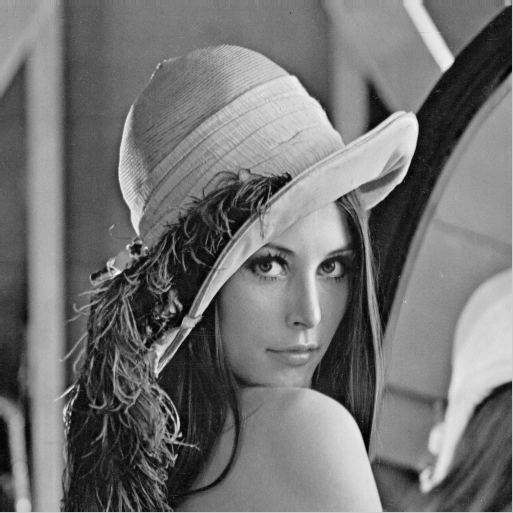
\includegraphics[scale=0.45]{comparison/original.PNG}
		\caption{Original image}
	\end{subfigure}
	\begin{subfigure}{0.49\textwidth} 
		\centering						
		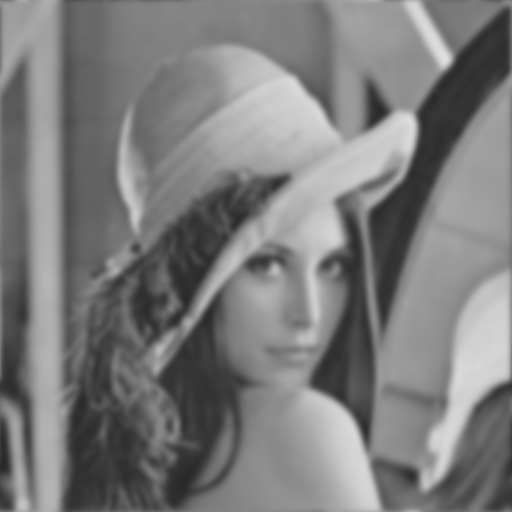
\includegraphics[scale=0.45]{comparison/gaussian.PNG}
		\caption{Blurred image with Gaussian $\sigma = 3$}
	\end{subfigure}\\
	\begin{subfigure}{0.49\textwidth} 
		\centering						
		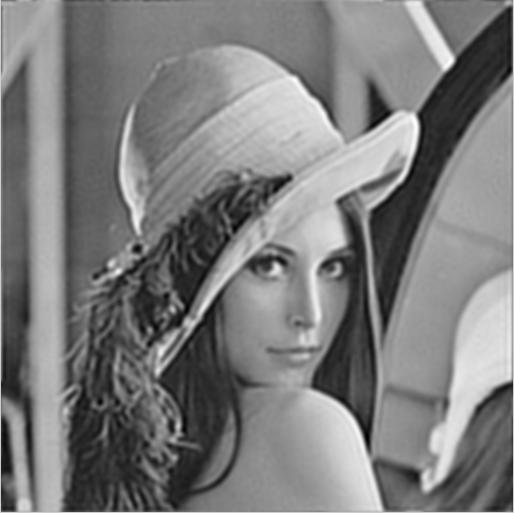
\includegraphics[scale=0.45]{comparison/energy1.PNG}
		\caption{Recovered image E1 $\lambda = 500$}
	\end{subfigure}
	\begin{subfigure}{0.49\textwidth} 
		\centering						
		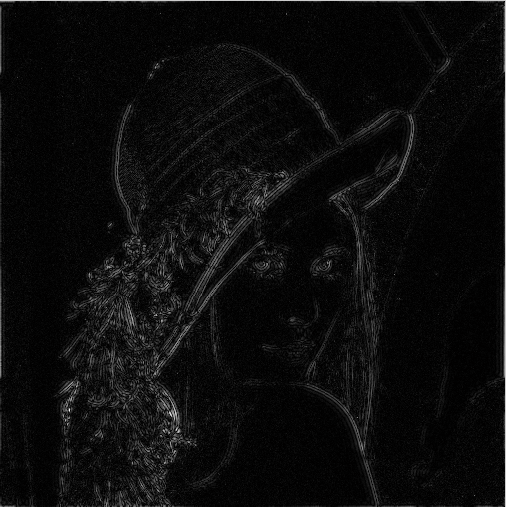
\includegraphics[scale=0.45]{comparison/difference1.PNG}
		\caption{Difference between original and E1 recovered}
	\end{subfigure}
	\begin{subfigure}{0.49\textwidth} 
		\centering						
		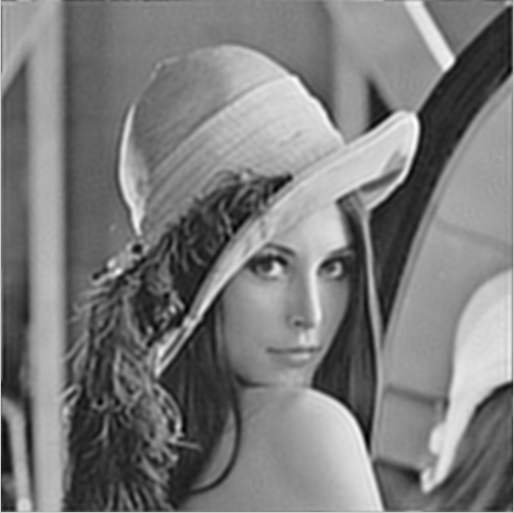
\includegraphics[scale=0.45]{comparison/energy2.PNG}
		\caption{Recovered image E2 $\lambda = 500$}
	\end{subfigure}
	\begin{subfigure}{0.49\textwidth} 
		\centering						
		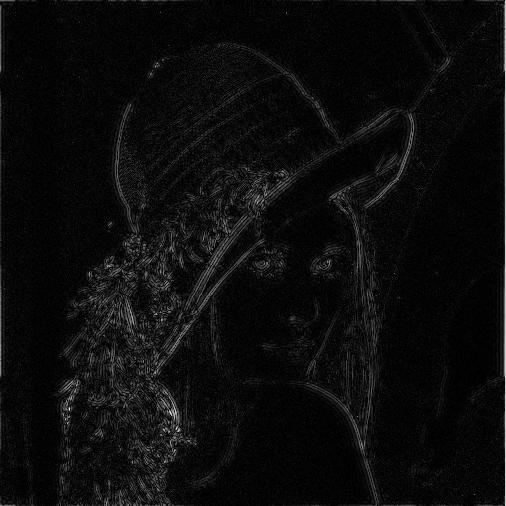
\includegraphics[scale=0.45]{comparison/difference2.PNG}
		\caption{Difference between original and E2 recovered}
	\end{subfigure}
	\begin{subfigure}{0.49\textwidth} 
		\centering						
		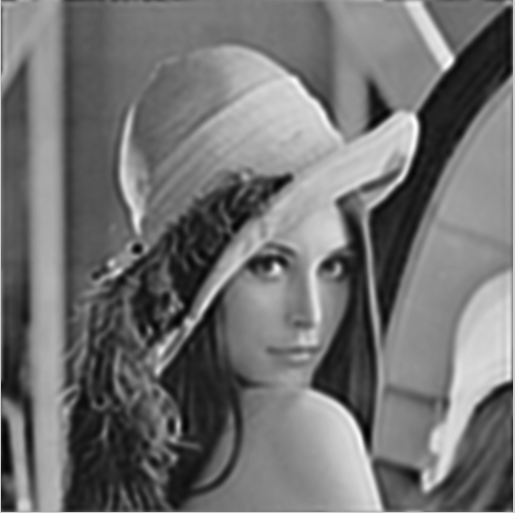
\includegraphics[scale=0.45]{comparison/lucy.PNG}
		\caption{Recovered image L-R method}
	\end{subfigure}
	\begin{subfigure}{0.49\textwidth} 
		\centering						
		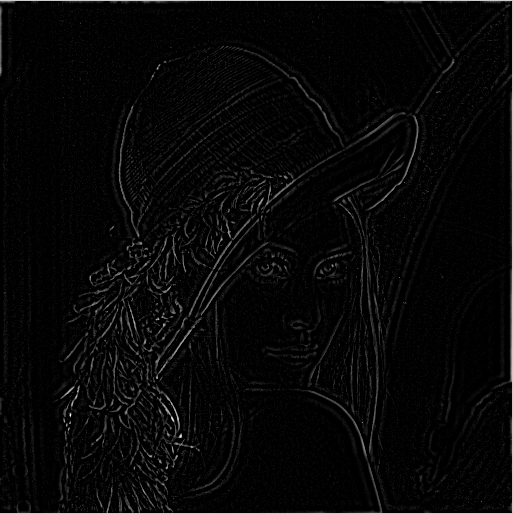
\includegraphics[scale=0.45]{comparison/difference3.PNG}
		\caption{Difference between original and L-R recovered}
	\end{subfigure}
	
	\caption{Comparison for different energies and Lucy-Richardson method}
	\label{comparison1}
\end{figure}
It is possible to check in the differences images that both of the energies perform practically in the same way (but it was expected to be more accurate for edges the second energy). Both of this methods had performed better than Lucy-Richarson method, it is easy to check by the level of detail in the differences images (i.e. the area of the eyes).

\section{Conclusions}
The methods give a good result when the kernel is known and there is no noise. \\
It is not an easy task the estimation of the parameter to regulate the ratio noise to signal. \\
Only some kind of noises (Gaussian, and sometimes S \& P) could be removed, and is really difficult in the case of strong noise. \\
When blur kernel is too high, as is not linear model, is impossible to recover the image with the methods proposed in this lab. 

%\begin{equation}
%I_{0}(x,y) = I(x,y)
%\end{equation} 
%\begin{equation}
%I_{n+1}(x,y) = \sum\limits_{i=-N}^N\sum\limits_{j=-N}^N w_{ij}I_{n}(x, y)/\sum\limits_{i=-N}^N\sum\limits_{j=-N}^N w_{ij} 
%\end{equation}
%\begin{equation}
%w_{ij} = exp \left(- \frac {dist^2(X_{0}, X_{ij})}{2*\sigma^2_{d}} - \frac{\left| I(X_{0})-I(X_{ij})\right|^2}{2*\sigma^2_{r}}\right)
%\end{equation}
%In this filter \textit{N} is the length of half of the size of a square patch that will be consider as the neighbourhood of the pixel to study, and it is proportionally related to $\sigma_{d}$.
%Several differences from the previous lab could be observed, the size of the neighbourhood won't be fixed, and the border to apply padding neither. The weight is depending in two exponential functions, allowing to consider with the most important influence the closer pixel and the intensity of such pixels. 
%The last parameter will be the number of iterations, in the case, \textit{n}. 
%
% \begin{figure}[H]
% 	%\centering
% 	\begin{subfigure}{0.29\textwidth} 						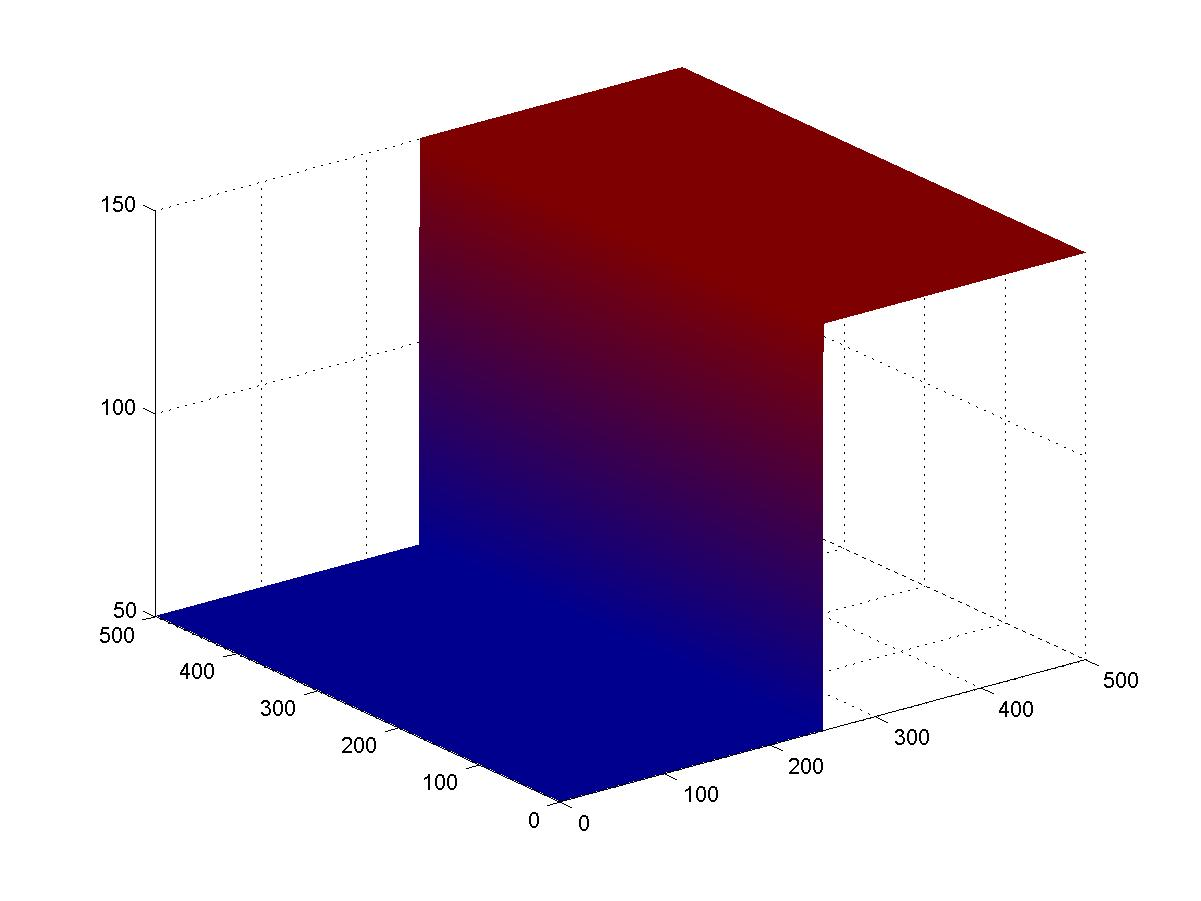
\includegraphics[scale=0.13]{original_1.JPG}
%		\caption{Original}
%	\end{subfigure}
%	\begin{subfigure}{0.29\textwidth} 						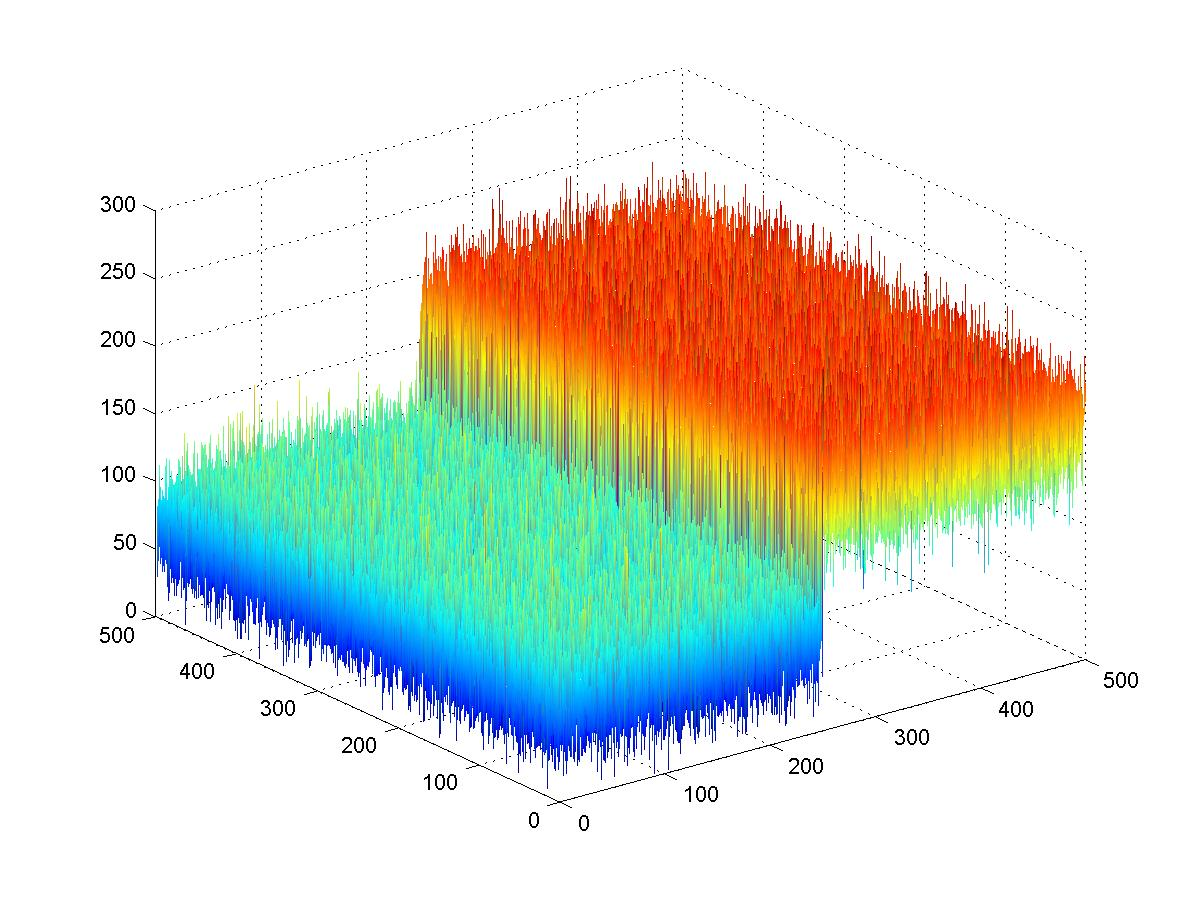
\includegraphics[scale=0.13]{noisy_1.JPG}
%		\caption{Noisy}
%	\end{subfigure}
%	\begin{subfigure}{0.29\textwidth} 						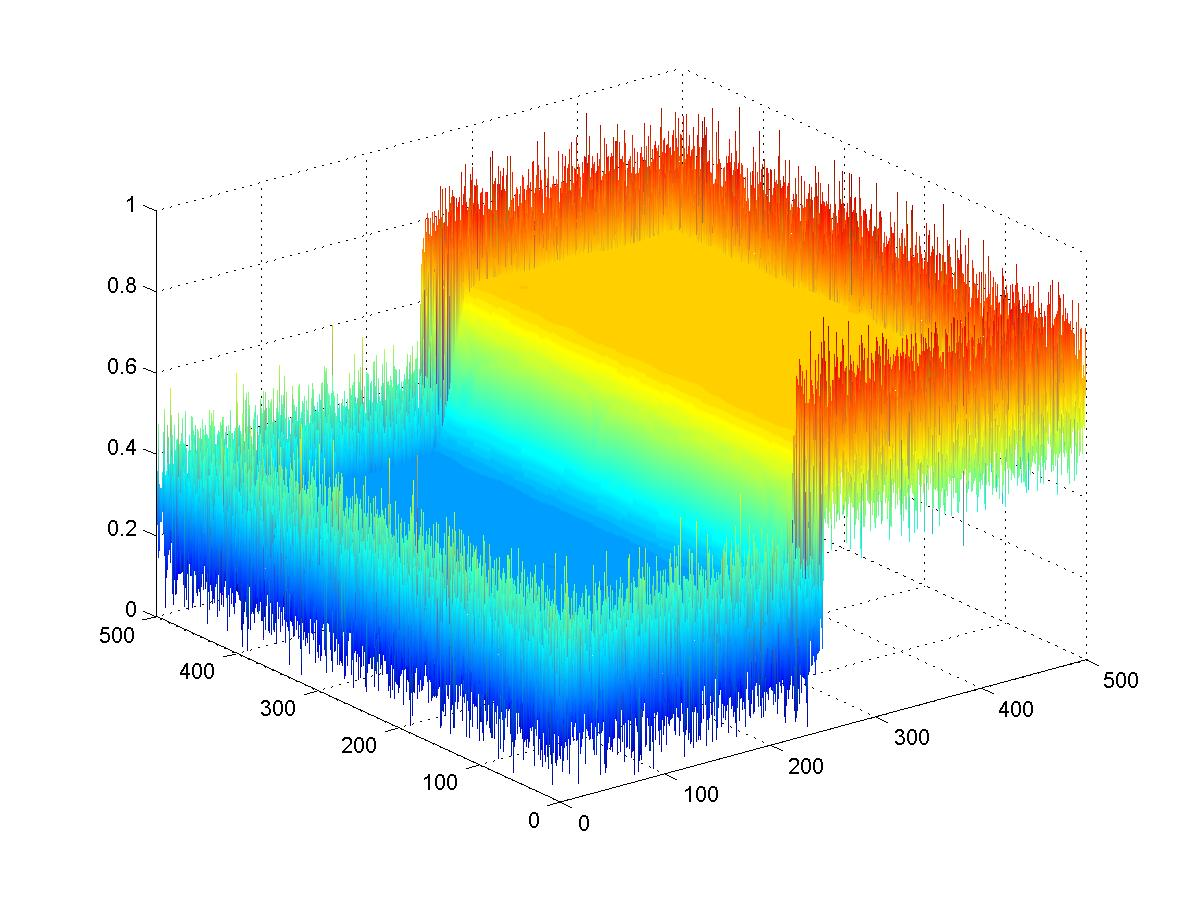
\includegraphics[scale=0.13]{filtered_1.JPG}
%		\caption{Filtered}
%	\end{subfigure}
%	\caption{Synthetic image filtered with bilateral filter}
%	\label{mesh}
%\end{figure}
% 
%
%\section{Evaluation and analysis}
%Once that the effect of the filter was checked over a synthetic image, would be nice to check how it works over a real image.
%\begin{figure}[H]
%	\centering
%	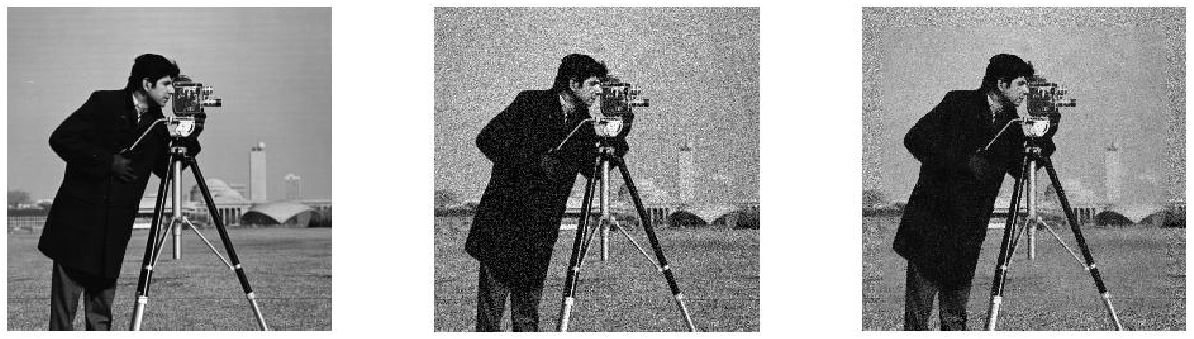
\includegraphics[width=1\textwidth]{camera_analysis.JPG} %
%	\caption{Bilateral filter with $\sigma_{d}=8, \sigma_{r}=10, iterations = 1$}
%	\label{camera}
%\end{figure}
%As it can be seen, the noise have been removed and edges are still remaining. It is also significant the size of the border, that of course, it not filtered. This padding problem could be partially solve mirroring the frame before applying the filter and cropping later on.    
%
%\subsection{Analysis of $\sigma_{r}$ variation}
%As the value of the parameter $\sigma_{r}$ is increased the filter will tend to be a regular average filter. This will be done by averaging with the same weight the neighbours that belong to the patch that contain as the central pixel the one that is being analysed. So the evolution of the blurring over the image could be seen in Fig.\ref{r} as this parameter changes.
%\begin{figure}[H]
%	\centering
%	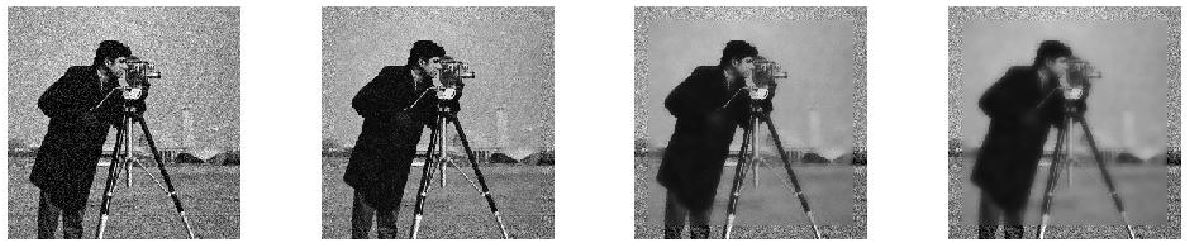
\includegraphics[width=1\textwidth]{sigmaR_analysis.JPG} %
%	\caption{Bilateral filter with $\sigma_{d}=75; \sigma_{r}=4, 10, 20; iterations = 1$}
%	\label{r}
%\end{figure}
%
%
%\subsection{Analysis of $\sigma_{d}$ variation}
%The effect of increasing the parameter related with the distances will affect in a similar way to the filter. It should be remarked that the bigger this value is the more will affect to the borders of the image. This is shown in Fig.\ref{d}. Adjusting these two first parameter would be possible to give more weight to the distances or to the intensities.
%\begin{figure}[H]
%	\centering
%	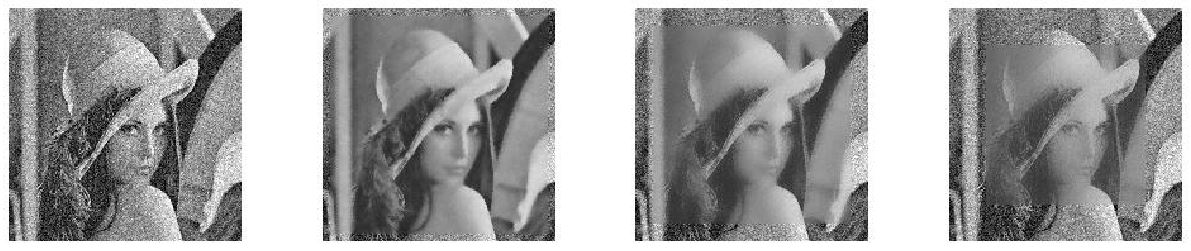
\includegraphics[width=1\textwidth]{sigmaD_analysis.JPG} %
%	\caption{Bilateral filter with $\sigma_{d}=25, 75, 125; \sigma_{r}=4; iterations = 1$}
%	\label{d}
%\end{figure}
%
%\subsection{Analysis of variation in the number of iterations}
%One of the advantages of this filter is that works pretty will even with just one iteration. The computational time will increase drastically as we the number of iterations rise.
%\begin{figure}[H]
%	\centering
%	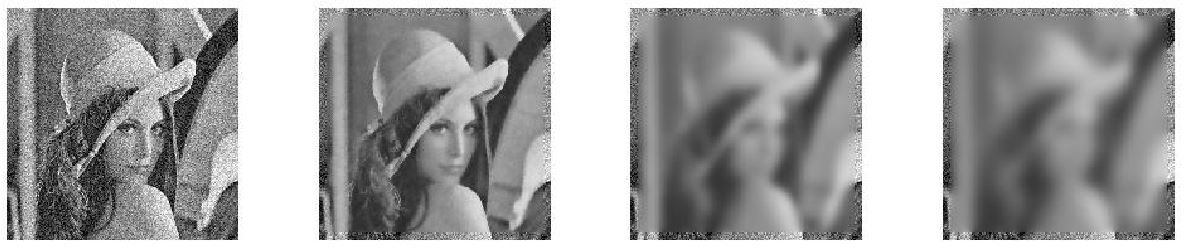
\includegraphics[width=1\textwidth]{iterations_analysis.JPG} %
%	\caption{Bilateral filter with $\sigma_{d}=75; \sigma_{r}=4; iterations = 1, 10, 20$}
%	\label{it}
%\end{figure}
%
%
%\subsection{Comparison of bilateral filter with non-local means filter}
%Non-local means considers that each pixel \textit{x} will have as neighbours any pixel \textit{y} which neighbourhood is similar to the neighbourhood of \textit{x}.
%\begin{equation}
%I(x) = \frac{1}{C(x)}\int_{\omega}e^{-\frac{1}{h^2}\int_{\Re^{2}} G_{\textit{a}}(t)\lvert u(x+t) -u(y-t) \rvert^{2}dt} u(y)dy 
%\end{equation}
%where $G_{\textit{a}}$ is a Gaussian kernel of standard deviation \textit{a} and \textit{h} as a filtering parameter.
%
%\begin{figure}[H]
%	\centering
%	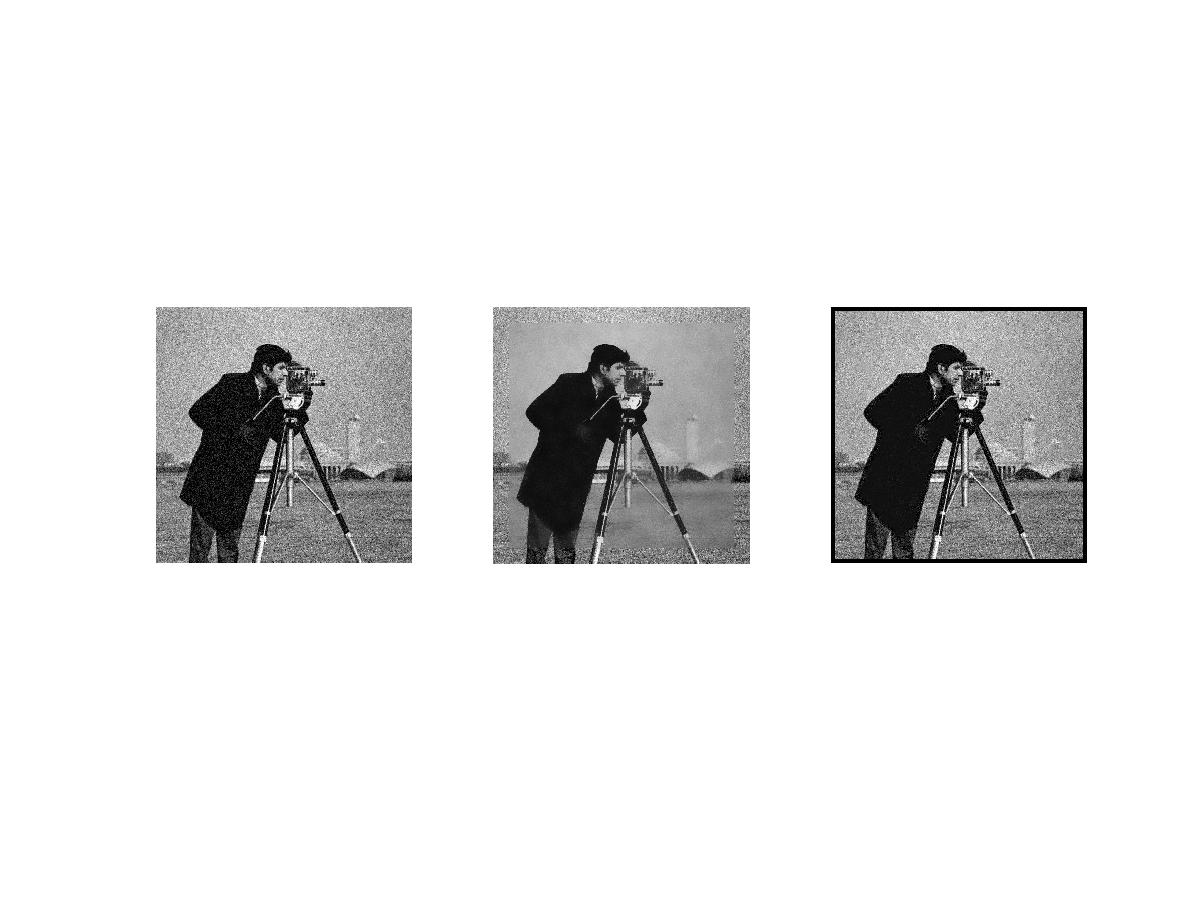
\includegraphics[width=1\textwidth]{bilateralVSnlmeans.JPG} %
%	\caption{Original noisy image. Bilateral filter with $\sigma_{d}=50; \sigma_{r}=4; iterations = 1$. NLMeans with $N = 9$}
%	\label{vs1}
%\end{figure}
%In Fig.\ref{vs1} a simpler version of the non-local means filter is used to compare with bilateral one. In a first instance is easy to check that the bilateral filter works much better in the preservation of the details (edges). The noise is also being removed in the non-local means filter. In the following pictures a deeper analysis will be performed. 
%\begin{figure}[H]
%	\centering
%	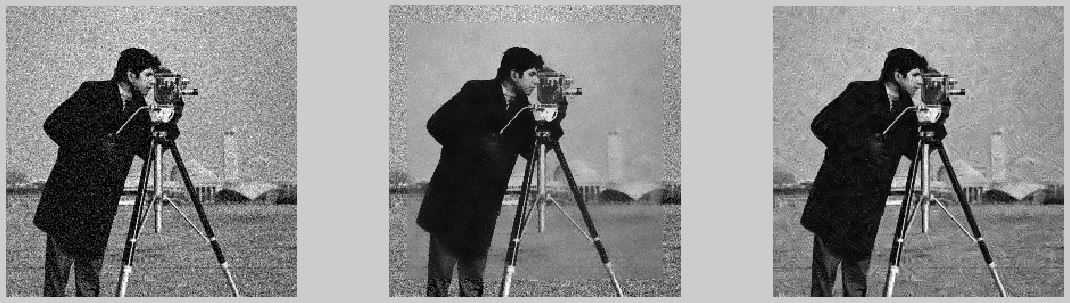
\includegraphics[width=1\textwidth]{bilateralVSnlmeans2.JPG} %
%	\caption{Original noisy image. Bilateral filter with $\sigma_{d}=50; \sigma_{r}=4; iterations = 1$.  NLMeans with $N = 9$}
%	\label{vs2}
%\end{figure}
%In this case a faster implementation of the non-local means has been used. In this case the edges are still better acquired by the bilateral filter but, non-local means seams to get more accurate grey levels.
%
%Let analyse, Fig.\ref{noise_comp} the subtraction of the filtered images in both cases to the noisy image.
%\begin{figure}[H]
%	\centering
%	
\includegraphics[width=1\textwidth]{noise_comparison.JPG} %
%	\caption{Original noisy. Noise after bilateral filter; Noise after non-local means filter}
%	\label{noise_comp}
%\end{figure} 
% 
%The information about the edges has been lost much more in the bilateral filter. The only area that has better results is the camera, where are very small lines in different directions limiting zones with relatively high contrast. This noise should be almost similar if the parameters are properly set up. Summing up, it could be said that these filters are much better than regular averaging or Gaussian ones for denoising purposes. The edges information remain in the filtered image and most of the noise has been removed.
  

\begin{thebibliography}{99}
%%

\bibitem{c1}
'Advanced Image Analysis Notes', Alexander Belyaev, Heriot Watt University, 2014
%%
%%\bibitem{c3}
%%'Ultrasound Image Enhancement Based on Image Compounding' - Yair Kerner - Technion (Israel Institute of Technology) - Haifa - June 2004 
%%
%%\bibitem{c4}
%%'Physical Principles of General and Vascular Sonography' - Jim Baun - San Francisco, CA -March 2009
%%
%%\bibitem{c5}
%%'Physical Principles of General and Vascular Sonography' - Jim Baun - San Francisco, CA -March 2009
%%
%%\bibitem{c6}
%%'Image Formation and Image Processing in Ultrasound' - Jeffrey C. Bamber - Institute of Cancer Research and The Royal Marsden NHS Trust, Surrey, SM2 5PT
\end{thebibliography}

\end{document}
